\chapter{Anhang}\label{Kapitel 6}
\section{Ergebnisse f"ur Linpack 100 und Whetstone auf dem RPi-Einzelrechner}\label{Ergebnisse_RPi}
\begin{verbatim}
##########################################
Unrolled Double Precision Linpack Benchmark - Linux Version in 'C/C++'

Optimisation Opt 3 32 Bit

norm resid      resid           machep         x[0]-1          x[n-1]-1
   1.7    7.41628980e-14   2.22044605e-16  -1.49880108e-14  -1.89848137e-14

Times are reported for matrices of order          100
1 pass times for array with leading dimension of  201

      dgefa      dgesl      total     Mflops       unit      ratio
    0.01613    0.00057    0.01669      41.14     0.0486     0.2981

Calculating matgen overhead
        10 times   0.01 seconds
       100 times   0.14 seconds
       200 times   0.28 seconds
       400 times   0.57 seconds
       800 times   1.13 seconds
Overhead for 1 matgen      0.00141 seconds

Calculating matgen/dgefa passes for 1 seconds
        10 times   0.17 seconds
        20 times   0.35 seconds
        40 times   0.70 seconds
        80 times   1.40 seconds
Passes used         57 

Times for array with leading dimension of 201

      dgefa      dgesl      total     Mflops       unit      ratio
    0.01609    0.00054    0.01663      41.29     0.0484     0.2970
    0.01603    0.00054    0.01658      41.43     0.0483     0.2960
    0.01610    0.00054    0.01664      41.25     0.0485     0.2972
    0.01609    0.00054    0.01663      41.29     0.0484     0.2970
    0.01603    0.00061    0.01663      41.28     0.0484     0.2970
Average                                41.31

Calculating matgen2 overhead
Overhead for 1 matgen      0.00137 seconds

Times for array with leading dimension of 200

      dgefa      dgesl      total     Mflops       unit      ratio
    0.01447    0.00054    0.01502      45.73     0.0437     0.2682
    0.01437    0.00051    0.01489      46.13     0.0434     0.2658
    0.01447    0.00051    0.01498      45.84     0.0436     0.2675
    0.01445    0.00051    0.01496      45.89     0.0436     0.2672
    0.01441    0.00051    0.01492      46.02     0.0435     0.2665
Average                                45.92

##########################################

From File /proc/cpuinfo
Processor : ARMv6-compatible processor rev 7 (v6l)
BogoMIPS  : 697.95
Features  : swp half thumb fastmult vfp edsp java tls 
CPU implementer	: 0x41
CPU architecture: 7
CPU variant	  : 0x0
CPU part	  : 0xb76
CPU revision	  : 7

Hardware	  : BCM2708
Revision	  : 000f
Serial		    : 00000000e98379f1


From File /proc/version
Linux version 3.6.11+ (dc4@dc4-arm-01) (gcc version 4.7.2 20120731 (prerelease) 
(crosstool-NG linaro-1.13.1+bzr2458 - Linaro GCC 2012.08) ) 
#538 PREEMPT Fri Aug 30 20:42:08 BST 2013


Unrolled Double  Precision       41.31 Mflops 

##############################################

##########################################
Single Precision C Whetstone Benchmark Opt 3 32 Bit, Sat Nov 30 15:22:14 2013

Calibrate
       0.04 Seconds          1   Passes (x 100)
       0.19 Seconds          5   Passes (x 100)
       0.96 Seconds         25   Passes (x 100)
       4.80 Seconds        125   Passes (x 100)

Use 260  passes (x 100)

From File /proc/cpuinfo
Processor : ARMv6-compatible processor rev 7 (v6l)
BogoMIPS  : 697.95
Features  : swp half thumb fastmult vfp edsp java tls 
CPU implementer	: 0x41
CPU architecture: 7
CPU variant	  : 0x0
CPU part	  : 0xb76
CPU revision	  : 7

Hardware	  : BCM2708
Revision	  : 000f
Serial		    : 00000000e98379f1


From File /proc/version
Linux version 3.6.11+ (dc4@dc4-arm-01) (gcc version 4.7.2 20120731 (prerelease) 
(crosstool-NG linaro-1.13.1+bzr2458 - Linaro GCC 2012.08) ) 
#538 PREEMPT Fri Aug 30 20:42:08 BST 2013


          Single Precision C/C++ Whetstone Benchmark

Loop content                  Result              MFLOPS      MOPS   Seconds

N1 floating point     -1.12475013732910156        97.643              0.051
N2 floating point     -1.12274742126464844       100.883              0.346
N3 if then else        1.00000000000000000                 690.831    0.039
N4 fixed point        12.00000000000000000                 423.573    0.193
N5 sin,cos etc.        0.49911010265350342                   5.050    4.284
N6 floating point      0.99999982118606567        86.081              1.629
N7 assignments         3.00000000000000000                 498.602    0.096
N8 exp,sqrt etc.       0.75110864639282227                   2.724    3.551

MWIPS                                            255.154             10.190

\end{verbatim}

\section{Shellskript zur Ausf"uhrung der Benchmarks auf n RPi-Nodes}\label{executeBenchmarksOnAllRPis.sh}

\endinput 

%Grafik aus PDF-File - diese Variante ist vorzuziehen, da sie die Einbundung echter Vektorgrafiken ermöglicht 
%\begin{figure}[htb]
%  \centering
%  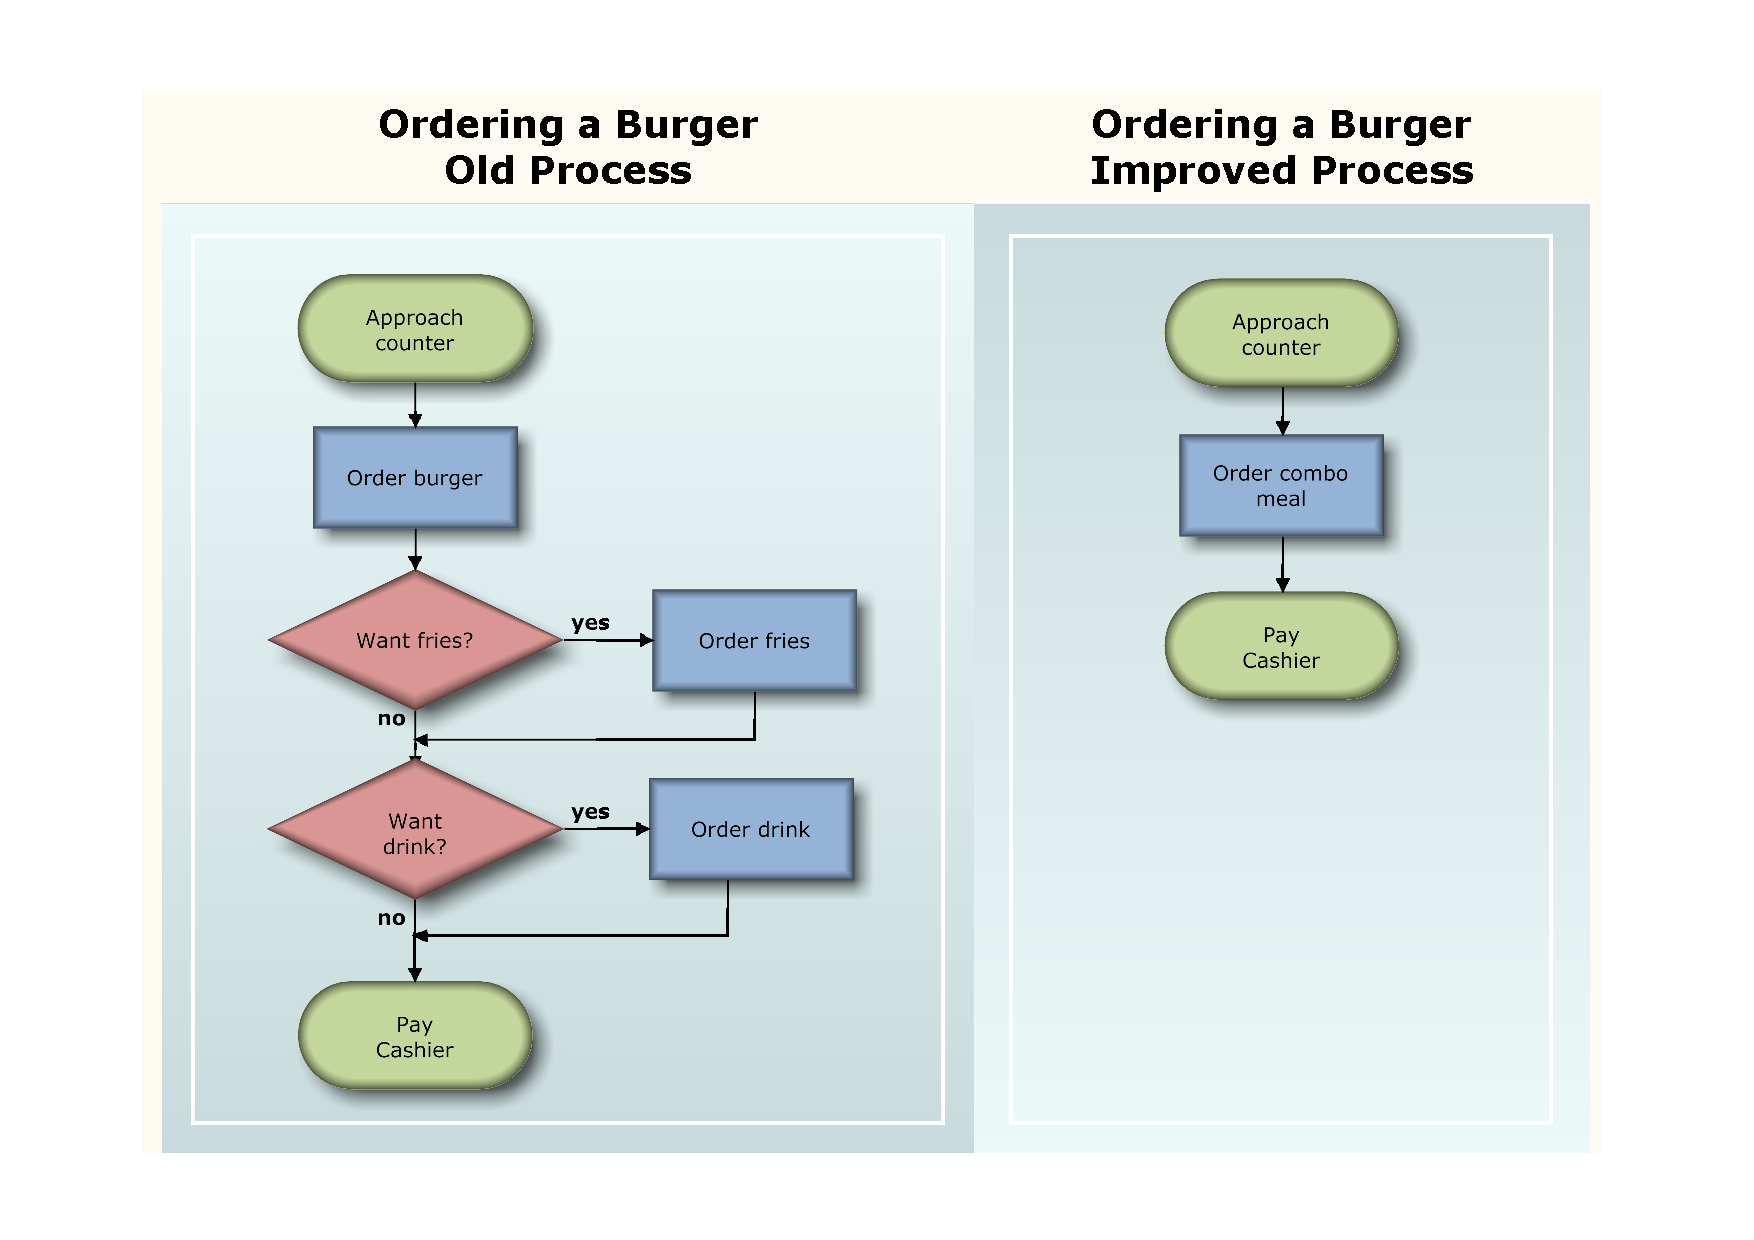
\includegraphics[scale=.6]{BurgerFlowchart}\\ % PDF-File
%  \caption{Donec tempor leo a massa \cite{scrguide07}}\label{fig:BurgerFlowchart}
%\end{figure}

